% ****** Start of file apssamp.tex ******
%
%   This file is part of the APS files in the REVTeX 4.1 distribution.
%   Version 4.1r of REVTeX, August 2010
%
%   Copyright (c) 2009, 2010 The American Physical Society.
%
%   See the REVTeX 4 README file for restrictions and more information.
%
% TeX'ing this file requires that you have AMS-LaTeX 2.0 installed
% as well as the rest of the prerequisites for REVTeX 4.1
%
% See the REVTeX 4 README file
% It also requires running BibTeX. The commands are as follows:
%
%  1)  latex apssamp.tex
%  2)  bibtex apssamp
%  3)  latex apssamp.tex
%  4)  latex apssamp.tex
%
\documentclass[aps,prl,showpacs,amsmath,amssymb,superscriptaddress]{revtex4-1}

%\documentclass[%
%reprint,
%superscriptaddress,
%groupedaddress,
%unsortedaddress,
%runinaddress,
%frontmatterverbose, 
%preprint,
%showpacs,preprintnumbers,
%nofootinbib,
%nobibnotes,
%bibnotes,
 %amsmath,amssymb,
 %aps,
%pra,
%prb,
%rmp,
%prstab,
%prstper,
%floatfix,
%]{revtex4-1}

\usepackage[titletoc]{appendix}
\usepackage{todonotes}
\usepackage{graphicx}% Include figure files
\usepackage{dcolumn}% Align table columns on decimal point
\usepackage{bm}% bold math
\usepackage{stmaryrd}
%\usepackage{hyperref}% add hypertext capabilities
%\usepackage[mathlines]{lineno}% Enable numbering of text and display math
%\linenumbers\relax % Commence numbering lines

%\usepackage[showframe,%Uncomment any one of the following lines to test 
%%scale=0.7, marginratio={1:1, 2:3}, ignoreall,% default settings
%%text={7in,10in},centering,
%%margin=1.5in,
%%total={6.5in,8.75in}, top=1.2in, left=0.9in, includefoot,
%%height=10in,a5paper,hmargin={3cm,0.8in},
%]{geometry}

\renewcommand{\AA}{\mathcal{A}}
\newcommand{\BB}{\mathcal{B}}
\newcommand{\DD}{\mathcal{D}}
\newcommand{\ff}{\mathbf{f}}
\newcommand{\nn}{\mathbf{n}}
\renewcommand{\tt}{\mathbf{t}}
\newcommand{\pderiv}[2]{\frac{\partial #1}{\partial #2}}
\newcommand{\rr}{\mathbf{r}}
\newcommand{\RR}{\mathbb{R}}
\renewcommand{\ss}{\mathbf{s}}
\renewcommand{\SS}{\mathcal{S}}
\newcommand{\TT}{\mathcal{T}}
\newcommand{\uu}{\mathbf{u}}
\newcommand{\WW}{\mathcal{W}}
\newcommand{\xx}{\mathbf{x}}
\newcommand{\xxi}{\boldsymbol{\xi}}
\newcommand{\yy}{\mathbf{y}}

\begin{document}

\preprint{APS/123-QED}

\title{Hydrodynamics and rheology of adhesive vesicle doublets}
% Force line breaks with \\
%\thanks{A footnote to the article title}%

\author{Bryan Quaife}
\affiliation{Department of Scientific Computing, Florida State University, Tallahassee, Florida, USA}
% \email{bquaife@fsu.edu}
% \altaffiliation[]{Department of Scientific Computing \\ Florida State University}
\author{Shravan Veerapaneni}%
% \email{shravan@umich.edu}
\affiliation{Department of Mathematics, University of Michigan, Ann Arbor, Michigan, USA}%
\author{Y.-N. Young}%
 \email[Corresponding author: ]{yyoung@njit.edu}
\affiliation{Department of Mathematical Sciences, Newark, NJ, USA}%

%\collaboration{MUSO Collaboration}%\noaffiliation

%\author{Charlie Author}
% \homepage{http://www.Second.institution.edu/~Charlie.Author}
%\affiliation{
% Second institution and/or address\\
% This line break forced% with \\
%}%
%\affiliation{
% Third institution, the second for Charlie Author
%}%
%\author{Delta Author}
%\affiliation{%
% Authors' institution and/or address\\
% This line break forced with \textbackslash\textbackslash
%}%
%
%\collaboration{CLEO Collaboration}%\noaffiliation

\date{\today}% It is always \today, today,
             %  but any date may be explicitly specified

\begin{abstract}

%\begin{description}
%\item[Usage]
%Secondary publications and information retrieval purposes.
%\item[PACS numbers]
%May be entered using the \verb+\pacs{#1}+ command.
%\item[Structure]
%You may use the \texttt{description} environment to structure your abstract;
%use the optional argument of the \verb+\item+ command to give the category of each item. 
%\end{description}
\end{abstract}

\pacs{Valid PACS appear here}% PACS, the Physics and Astronomy
                             % Classification Scheme.
%\keywords{Suggested keywords}%Use showkeys class option if keyword
                              %display desired
\maketitle

%\tableofcontents

%%%%%%%%%%%%%%%%%%%%%%%%%%%%%%%%%%%%%%%%%%%%%%%%%%%%%%%%%%%%%%%%%%%%%%%%

\todo[inline]{$\sigma$ is overdefined as the Hamacher constant, and the
tension, and possibly the stress.  Replace Hamacher constant with $H$.}

\todo[inline]{In the xtensional flow, put a plus sign after the 0.
Indicate the flow with arrows.  Do the same for the shear and Figure 9
(right).}

\section{Introduction}
Vesicles (closed fluid-filled phospholipid bilayer membranes) have been widely utilized
as biological cell mimics in biophysics and material engineering \cite{}. 
%
The ever expanding applications have encouraged detailed experimental, theoretical and numerical investigations of vesicle hydrodynamics
in applied flow, electric and magnetic fields. Theoretical investigations often take the form of small-deformation analysis or spheroidal dynamics of a nearly-spherical vesicle (or nearly-circular in two dimensions) subjected to an applied flow or under an external forcing \cite{Barthes-BieselRallison1981_JFM,Misbah2006_PRL,Vlahovska2007_PRE,Finken2008_EPL,ZhangZahnTanLin2013_PoF,Nganguia2013_PRE}. 
On the other hand, various numerical methods have been developed for simulating the transient hydrodynamics of vesicle suspensions  \cite{BagchiJohoson2005_JBE,Biben2005_EJP,Veerapaneni2009_JCP,SeolHuKimLai2016_JCP}.  
%Experiments are performed to study vesicle hydrodynamics under various flowing conditions or forcing configurations \cite{MaderVitkova2006_EurPhysJE, Abkarian2008_SoftMatt,DahlNarsimhanGouveia2016_SoftMatt}. 
Collective vesicle hydrodynamics naturally is dictated by the individual vesicle-vesicle interactions;  for example, 
it was shown recently that vesicles may align to form chains along the direction of the externally applied DC electric field with ensuing consequences to suspension rheology \cite{wu2018pairwise}.

In numerical simulations of vesicle suspensions, it is often assumed that the lubrication layer between vesicle membranes acts to keep the 
membrane-membrane interaction, such as the van der Waals type interaction, negligible. However the amphiphilic natures of lipid molecules (a hydrophobic tail and a hydrophilic head with an electric dipole) complicate the interactions between a lipid bilayer membrane and a solid (such as a glass substrate or a nano particle) or another bilayer membrane \cite{EvansMetcalfe1984_BJ,Book_PhysicalBasisCellAdhesion,Book_IntermolecularSurfaceForces}.
Studies confirmed that such interaction potential inevitably consists of a long-range attraction component and a short-range repulsion component 
\cite{Book_IntermolecularSurfaceForces}. Such interactions leads to adhesion at the separation distance that minimizes the
interaction potential \cite{Book_IntermolecularSurfaceForces}, and are essential in many biomedical, biological and biophysical processes.
For example, vesicle adhesion is essential for membrane fusion/fission in endocytosis and exocytosis, the transport of small
vesicles through membrane surfaces.

%
Adhesion between a vesicle and a substrate has been extensively studied, primarily focused on analyzing the static equilibrium shapes \cite{Seifert1990_PRA, ShiFengGao2006_ActaMechSin, LinFreund2007_IntJSolidsStructures, das2008adhesion, zhang2009phase} than the the transient adhesion process; exceptions include \cite{cantat1999lift, suk-sei2001, BlountMiksisDavis2013_PRSa}.
Adhesion between bilayer membranes was first experimentally observed by Evans and Metcalfe \cite{EvansMetcalfe1984_BJ}, who measured 
the reduction in the free energy per unit area of membrane-membrane contact formation due to the Van der Waals' attraction. For a membrane-membrane
separation distance of $\sim 3$ nm, they estimated that the Hamaker constant is approximately $5.8\times 10^{-14}$ ergs, which corresponds to an adhesion energy density around $1$ mJ/m$^2$. The ratio of adhesion energy per unit area to the bending energy (bending rigidity of lipid bilayer membranes $\sim 10^{-19}$ J) gives a measure of vesicle deformation in the presence of adhesion \cite{RamachandranAndersonLealIsraelachvili2010_Langmuir}. In this work we focus on regimes where the ratio is of order unity, between the weak adhesion (ratio $\ll 1$) and strong adhesion (ratio $\gg 1$) regimes. 
In this regime the membrane deformation may increase the ``contact
area'' between two vesicles and enhance the adhesion effects. The
equilibration of vesicle membranes under adhesion in these regimes have
been well studied and documented
(see~\cite{RamachandranAndersonLealIsraelachvili2010_Langmuir} and
references therein). However it is unclear how the adhesion couples to
the vesicle hydrodynamics in such regime.  Our work in this paper aims
to address this question with quantitative characterization in terms of
physical parameters.


%Hydrodynamics of a single vesicle in Stokes flow has been extensively investigated. In a planar shear flow, the vesicle hydrodynamics is characterized by
%excess area (reduced volume), viscosity contrast between interior and exterior fluids, and shear rate of the imposed far-field fluid flow. In addition a vesicle
%with a rigid particle inside is also investigated as a biological mimic of a 
%eukaryotic cell with a nucleus that occupies nearly half of the intracellular volume \cite{Veerapaneni2011_PRL}. Small-deformation analysis shows that
%a vesicle tank-treads in a planar shear flow for low viscosity contrast and shear rate. At high viscosity contrast the tank-tread (TT) dynamics transitions to tumbling (TB) \cite{Misbah2006_PRL,Vlahovska2007_PRE} ,
%and this leads to a transition in effective shear viscosity in the vesicle suspension \cite{Misbah2006_PRL,Vitkova2008_BJ} that is also validated
%by direct numerical simulations \cite{GhigliottiBibenMisbah2010_JFM} and experiments \cite{KantslerSegreSteinberg2008_EPL,ZabuskySegreDeschamps2011_PoF}.
%Between TT and TB vesicle hydrodynamics, a breathing (tremble) is also observed \cite{Misbah2006_PRL,KantslerSegreSteinberg2008_PRL,ZhaoShaqfeh2011_JFM,SpannZhaoShaqfeh2014_PoF} to affect the effective shear viscosity in a 
%different way.
%
%In an extensional flow (planar or uniaxial), vesicle shape dynamics
%depends sensitively on the vesicle reduced volume  and the elastic capillary number \cite{KantslerSegreSteinberg2008_PRL,ZhaoShaqfeh2013_JFM,Narsimhan2014_JFM,DahlNarsimhanGouveia2016_SoftMatt}: Asymmetric shape and oscillatory undulation of the vesicle membrane are two examples of the complex vesicle hydrodynamics in an extensional flow.

In a quiescent environment, sub-micron size vesicles are found to form a
doublet due to their Van der Waals' attractive
interactions~\cite{RamachandranAndersonLealIsraelachvili2010_Langmuir}.
Due to the strong Van der Waals' adhesive force, the vesicles are far
from spherical shape and the membrane is almost flat in the ``contact"
region. Gires {\it et al.} used small-deformation analysis to
investigate the hydrodynamic interactions between two vesicles in a
planar shear flow with a long separation distance
\cite{GiresDankerMisbah2012_PRE}. They found that the vesicle
interaction could be either attractive or repulsive depending on the
organization of the two vesicles relative to the shear flow. To the best
of authors' knowledge, the effects of close-range vesicle adhesion on
their hydrodynamics under an external flow have not been studied and
quantified. The goal of this work is to use state-of-the-art boundary
integral simulations to numerically investigate the dynamics of two
vesicles in both planar shear flow and extensional flow for a wide range
of vesicle shapes and adhesive strength and distance.


Boundary integral equation (BIE) approaches are well-suited for solving the low Re flow problems considered here as they lead to reduction in dimensionality and 
achieve high-order accuracy even for moving geometry problems. When the vesicles adhere, one major issue for BIE solvers is to resolve the vesicle-vesicle hydrodynamic forces which become 
{\em nearly singular}. In this work, we use the recently developed spectrally-accurate algorithm of \cite{barnett2015spectrally} for overcoming this problem. To overcome the numerical stiffness induced by the membrane bending forces, 
we extend the adaptive time-stepping scheme developed in \cite{quaife2016adaptive} to our setting. 

This paper is organized as follows.




%%%%%%%%%%%%%%%%%%%%%%%%%%%%%%%%%%%%%%%%%%%%%%%%%%%%%%%%%%%%%%%%%%%%%%%%
\section{Governing Equations}
We consider suspensions of locally inextensible vesicles in an unbounded
two-dimensional viscous fluid.  For simplicity, we assume the fluid
viscosity both inside and outside the vesicles is constant, but our
method can be easily adjusted to account for a viscosity contrast.
Individual vesicles are denoted as $\gamma_j$, and they are
parameterized in arclength as $\xx_j(s,t)$.  The union of all vesicles
is denoted by $\gamma$.  Given a background velocity $\uu_\infty$, the
governing equations are
\begin{equation*}
\begin{aligned}
  \mu \Delta \uu = \nabla p, \quad &\xx \in \RR^2,
    &&\mbox{\em conservation of momentum} \\
  \nabla \cdot \uu = 0, \quad &\xx \in \RR^2, 
    &&\mbox{\em conservation of mass} \\
  \uu \rightarrow \uu_\infty, \quad &\|\xx\| \rightarrow \infty,
    &&\mbox{\em far-field condition} \\
  \uu(\xx,t) = \dot{\xx}, \quad &\xx \in \gamma,
    &&\mbox{\em velocity continuity} \\
  \xx_s \cdot \uu_s =0, \quad &\xx \in \gamma,
    &&\mbox{\em vesicle inextensibility} \\
  \llbracket T \rrbracket \nn = \xxi, \quad &\xx \in \gamma,
    &&\mbox{\em non-zero traction jump}
\end{aligned}
\end{equation*}
where $\xxi$ is the traction jump that depends on a bending, stretching,
and adhesion.  The bending term is $\BB \xx = -\kappa_b \xx_{ssss}$,
where $\kappa_b$ is the bending modulus, and this term comes from the
Helfrich energy.  For the numerical examples, we set $\kappa_b = 1$ and
use a Hamaker constants ranging from $0.1$ to $1$.  The stretching term
is $\TT \sigma  = (\sigma \xx_s)_s$, where $\sigma$ is the tension.  The
resistance to bending and stretching are standard assumptions of
vesicles.  In this work, we include an adhesive term, $\AA \xx$, that we
now describe.

%%%%%%%%%%%%%%%%%%%%%%%%%%%%%%%%%%%%%%%%%%%%%%%%%%%%%%%%%%%%%%%%%%%%%%%%
\subsection{Adhesion Model}
The adhesion model of Sukumaran and Seifert~\cite{suk-sei2001} considers adhesion
between a single three-dimensional vesicle and a solid wall at $z=0$.
\todo[inline]{Need a cartoon picture in here.  Some kind of version of
the one I had for my SIAM Life Sciences Talk}
The adhesion potential in their model is of the functional form in equation~\ref{eq:adhesion_potential} with $(m,n) = (4,2)$:
\begin{align}
\label{eq:adhesion_potential}
  \phi(z) = \sigma \left[ 
    \left(\frac{\delta}{z}\right)^m - \frac{m}{n} \left(\frac{\delta}{z}\right)^n \right],
\end{align}
where $z$ is the distance between the solid wall and the vesicle,
$\sigma$ is the Hamaker constant, and $\delta$ is the adhesion length
scale.  We generalize this model to an unbounded suspension of vesicles.
We assume that the adhesion force applies between all pairs of points on
different vesicles, so we are interested in Hamaker constants that are
appropriate for lipid-lipid interactions. In
Appendix~\ref{sec:appendixA}, the adhesive force at a point $\xx$ on
vesicle $j$ is shown to be
\begin{align}
  \AA\xx:=-\sigma m \delta^{n}\sum_{\substack{k=1 \\ k \neq j}}^M 
  \int_{\gamma_k} \frac{\xx - \yy}{\|\xx - \yy\|^{m+2}} 
  \left(\delta^{m-n} - \|\xx - \yy\|^{m-n} \right) ds_\yy.
  \label{eqn:adhesionForce}
\end{align}

%\begin{align}
%  \AA\xx:=-4 \sigma \delta^2\sum_{\substack{k=1 \\ k \neq j}}^M 
%  \int_{\gamma_k} \frac{\xx - \yy}{\|\xx - \yy\|^6} 
%  \left(\delta^2 - \|\xx - \yy\|^2 \right) ds_\yy.
%  \label{eqn:adhesionForce}
%\end{align}

The exponents $(m,n)$ depend on the geometry of the two objects under adhesion \cite{Book_IntermolecularSurfaceForces}: $(m,n)=(4,2)$ corresponds to two
flat, planar surfaces interacting with each under a long-range attraction and a short-range repulsion. On the other hand, $(m,n) = (12,6)$ corresponds to the L-J potential between
two molecules. The adhesion potential in  the integral of equation~\ref{eqn:adhesionForce} is between two small patches of lipid bilayer membrane. Thus we argue that
a reasonable choice for $(m,n)$ is between $(m,n) = (4,2)$ and $(m,n) = (12,6)$. 


%%%%%%%%%%%%%%%%%%%%%%%%%%%%%%%%%%%%%%%%%%%%%%%%%%%%%%%%%%%%%%%%%%%%%%%%
\subsection{Integral Equation Formulation}
Because the fluid equations are linear and elliptic, an integral
equation formulation is possible.  This has several advantages,
including that only the vesicle interfaces require discretization.  We
start by defining the Stokes single-layer potential
\begin{align}
  \SS[\ff](\xx) &= \frac{1}{4\pi\mu} \int_\gamma \left(
    -\log \rho + \frac{\rr \otimes \rr}{\rho^2} \right) 
    \ff(\yy) ds_\yy, \quad \xx \in \RR^2,
  \label{eqn:SLP}
\end{align}
where $\rr = \xx - \yy$ and $\rho = \|\rr\|$.  The traction jump of the
velocity $\uu(\xx) = \SS[\ff](\xx)$ is the density function $\ff$, so
the fluid velocity is $\xx \in \RR^2$ is
\begin{align*}
  \uu(\xx) = \uu_{\infty}(\xx) + \SS[\xxi](\xx).
\end{align*}
The traction jump is given by three terms: the bending, tension, and
adhesion.  Therefore
\begin{align*}
  \xxi = -\kappa_b \xx_{ssss} + (\sigma \xx_s)_s + \AA \xx.
\end{align*}
Applying the no-slip boundary condition on each vesicle, the governing
equations are
\begin{align*}
  &\dot{\xx} = \uu_{\infty}(\xx) + \SS[\xxi](\xx), \\
  &\xx_s \cdot \uu_s = 0, \\
  &\xxi = -\kappa_b \xx_{ssss} + (\sigma \xx_s)_s + \AA\xx.
\end{align*}
Defining the bending operator as $\BB[\xx](\ff) = -\kappa_b \ff_{ssss}$,
and the tension operator $\TT[\xx](\sigma) = (\sigma \xx_s)_s$, the
no-slip boundary condition can be written as
\begin{align*}
  \pderiv{\xx}{t} = \SS \BB \xx + \SS \TT \sigma + \SS \AA \xx.
\end{align*}
We apply the IMEX-Euler method 
\begin{align*}
  \frac{\xx^{N+1} - \xx^N}{\Delta t} = \SS^N \BB^N \xx^{N+1} + 
  \SS^N \TT^N \sigma^{N+1} + \SS^N \AA^N \xx^N,
\end{align*}
that treats both the bending and tension terms
semi-implicitly~\cite{qua-bir2014}. Note that the adhesive term is
treated explicitly.  Therefore, a single time step requires solving
\begin{align}
  \xx^{N+1} - \Delta t \SS^N \BB^N \xx^{N+1} - 
    \Delta t \SS^N \TT^N \sigma^{N+1} = \xx^N + 
    \Delta t \SS^N \AA^N \xx^N,
  \label{eqn:IMEXEuler}
\end{align}
along with the inextensibility constraint that is discretized as
\begin{align*}
  \xx_s^{N} \cdot \xx_{s}^{N+1} = 1.
\end{align*}
We discretize the vesicles at a set of collocation points, compute the
bending and tension terms with Fourier differentiation, and apply
Alpert quadrature to the logarithmically singular single-layer potential
$\SS$~\cite{alp1999}.  The source and target points of the adhesion
force never coincide since they are always on different vesicles, so the
adhesion force~\eqref{eqn:adhesionForce} is computed with the spectrally
accurate trapezoid rule~\cite{tre-wei2014}.  To control the error and
achieve higher-order accuracy in time, we apply a time adaptive spectral
deferred correction method~\cite{qua-bir2016}.  The SDC method is able
to achieve second-order accuracy by iteratively applying the first-order
method~\eqref{eqn:IMEXEuler}.


%%%%%%%%%%%%%%%%%%%%%%%%%%%%%%%%%%%%%%%%%%%%%%%%%%%%%%%%%%%%%%%%%%%%%%%%
\subsection{The Shear and Normal Stresses}
Consider a single vesicle $\gamma$ and a target point $\xx$ in the fluid
bulk.  In addition to the velocity $\uu$, we are also interested in
computing the shear stress and normal stresses of each vesicle.
Therefore, we must compute the total stress tensor
\begin{align*}
  T = - p I + \nabla \uu + \nabla \uu^T
\end{align*}
of the single-layer potential~\eqref{eqn:SLP}.  Given a traction jump
$\xxi$ across a vesicle $\gamma$, the velocity, pressure, and stress
tensor at a target point $\xx$ are in the bulk
\begin{align*}
  \uu(\xx) &= \SS_\uu[\xxi](\xx) = \frac{1}{4\pi\mu}\int_{\gamma} \left( 
    -\log \rho + \frac{\rr \otimes \rr}{\rho^2} \right) 
    \xxi ds_\yy, \\
    p(\xx) &= \SS_p[\xxi](\xx) = \frac{1}{2\pi} \int_{\gamma} 
    \frac{\rr \cdot \xxi}{\rho^2} ds_\yy, \\
    T(\xx) &= \SS_T[\xxi](\xx) = -\frac{1}{\pi}\int_{\gamma}
      \frac{\rr \cdot \xxi}{\rho^2} 
      \frac{\rr \otimes \rr}{\rho^2} ds_\yy.
\end{align*}
We require the stress tensor on the vesicle, and the layer potential for
$\SS_T$ has a jump as $\xx$ approaches $\gamma$.  Accounting for the
jump, the stress tensor at $\xx \in \gamma$ is
\begin{align*}
  T(\xx) = \frac{1}{2}(\nn \otimes \xxi) + \frac{1}{2} \left(
    \tt \otimes \left[
    \begin{array}{cc}
      2 t_x t_y & t_y^2 - t_x^2 \\
      t_y^2 - t_x^2 & -2 t_x t_y
    \end{array}
    \right] \xxi \right) + 
  \SS_T[\xxi](\xx).
\end{align*}
With the stress tensor computed for $\xx \in \gamma$, we can compute the
shear stress and normal stress
\begin{align*}
  \tau^\tt = (T \nn) \cdot \tt, \qquad
  \tau^\nn = (T \nn) \cdot \nn.
\end{align*}

%%%%%%%%%%%%%%%%%%%%%%%%%%%%%%%%%%%%%%%%%%%%%%%%%%%%%%%%%%%%%%%%%%%%%%%%
\section{Adhesion of two vesicles in a quiescent flow} 
\label{sec:qflow} 

When two vesicles move towards (or away from) each other under a constant force $F$ without any external fluid flow, the height  $(h)$ of the thin liquid film between two vesicles follows the
draining dynamics \cite{RamachandranLeal2010_PoF}
\begin{equation}
\label{eq:dhdt}
\frac{d h}{dt} \sim \frac{K_a^{2/3} F^{1/3}}{\mu R_0^{10/3}} h^3,
\end{equation}
where $K_a$ is the area expansion modulus, $\mu$ is the viscosity of exterior fluid, $R_0$ is the radius of the undeformed vesicle.
For the case of a constant forcing $F$ (independent of separation distance $h$ and time $t$), equation~\ref{eq:dhdt} can be easily integrated to give
a relation between film thickness $h$ and time $t$:
\begin{equation}
t \sim \frac{\mu R_0^{10/3}}{K_a^{2/3} F^{1/3}}\frac{1}{2 h^2} \bigg|^{h(t)}_{h(0)},
\end{equation}
where $h(0)$ is the vesicle separation at $t=0$.
We note that $F< (>) 0$ for an attractive  (repulsive) interaction between two vesicles,  and consequently $h(t)$ decreases (increases) from  the initial separation distance $h(0)$. 
When the force is attractive, $h$ decreases monotonically and $t$ in the above
equation is the
draining time that diverges as $h\rightarrow 0$.
%Similarly $F>0$ for a repulsive force and consequently $h(t) > h(0)$.

When the force on each vesicle is a function of separation distance $h$ of the form (with an integer $m\ge 2$)
\begin{equation}
\label{eq:Fh}
F(h) \sim \sigma \frac{\delta^m}{h^{m+1}}\left(\left(\frac{\delta}{h}\right)^2-1\right),
\end{equation}
attraction is dominant at ``large" scales ($h > \delta$) while repulsion is dominant at ``small" scales ($h<\delta$).
Integration of equation~\ref{eq:dhdt} with the above $F(h)$ gives the relationship between $t$ and $h$.
In this case the relationship involves an integral of a function of dimensionless $\bar{h} \equiv h/\delta$:
\begin{align}
t\frac{K_a^{2/3}}{\mu R_0^{10/3}}& = \int^{h(t)}_{h(0)}-\frac{dh}{h^3 F^{1/3}} = -\frac{1}{\sigma^{1/3}\delta^{5/3}}\int^{\bar{h}(t)}_{\bar{h}(0)}\frac{d \bar{h}}{\bar{h}^{(8-m)/3}(\bar{h}^2-1)^{1/3}},
\end{align}
\begin{equation}
\label{eq:teq_scaling}
t\sim \frac{\mu R_0^{10/3}}{K_a^{2/3}}\frac{1}{\sigma^{1/3}\delta^{5/3}}.
\end{equation}
Equation~\ref{eq:teq_scaling} tells us that both adhesion strength $\sigma$ and the separation distance $\delta$ affect
the time it takes for a pair of vesicles to reach equilibrium under adhesion force $F$ in equation~\ref{eq:Fh}.  In particular, the equilibration time $t$ 
is proportional to (1) the separation distance $\delta^{-5/3}$ (thus $t\rightarrow \infty$ as $\delta\rightarrow 0$), and (2) the adhesion strength $\sigma^{-1/3}$ 
(as in constant forcing case \cite{RamachandranLeal2010_PoF}).  From the above analysis we also expect that the scaling of $t$ with respect to $\delta$ depends on the
adhesion potential, while the scaling with respect to adhesion strength is independent of the specific form of the potential.

\begin{figure}
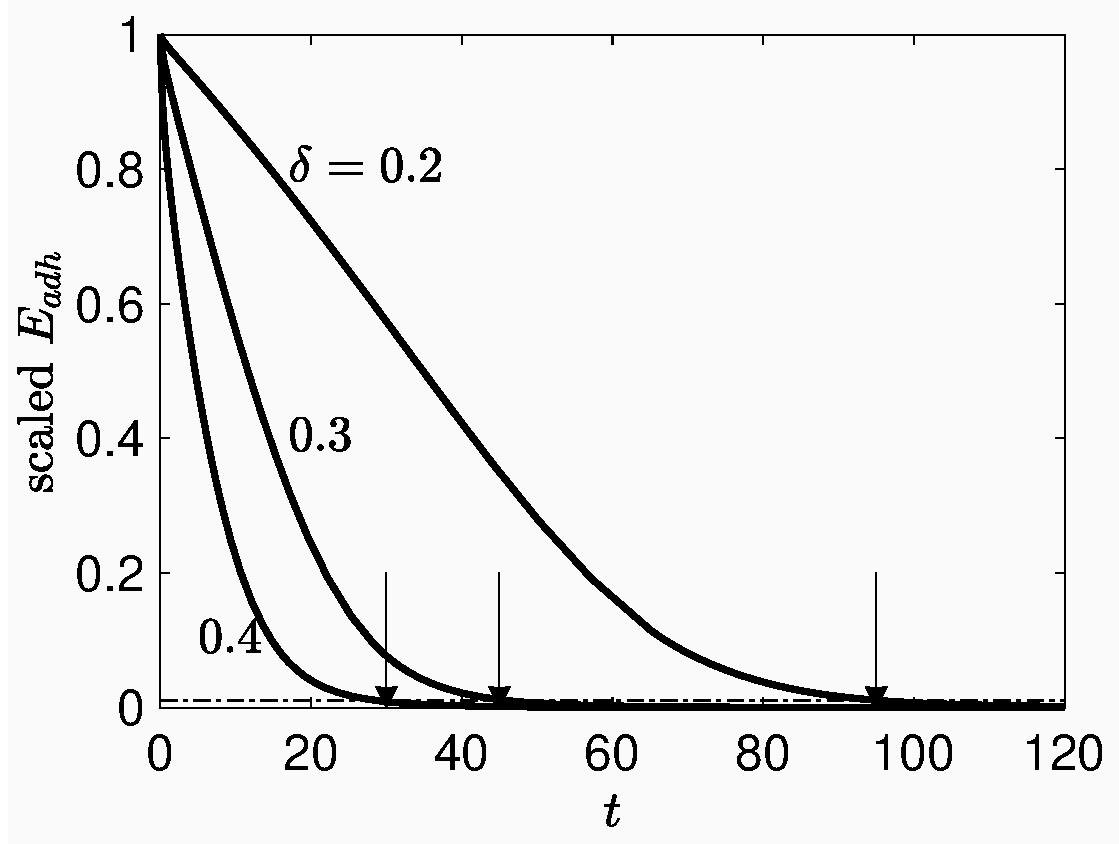
\includegraphics[keepaspectratio=true,scale=0.4]{figs/Dec13a_time_scaling01.eps}
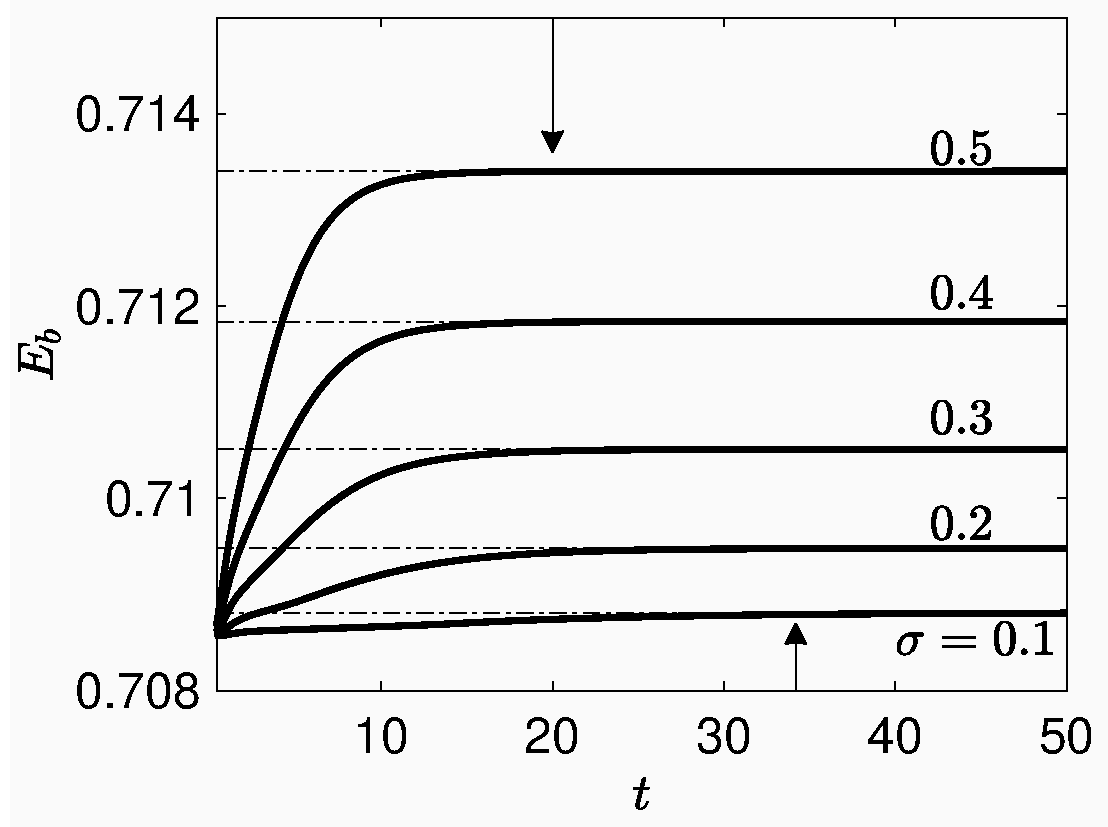
\includegraphics[keepaspectratio=true,scale=0.4]{figs/Dec13a_time_scaling02.eps}
\caption{Scaling of the time it takes for two vesicles to reach equilibrium: (a) scaling with respect to $\delta$ with $\sigma=0.1$, and (b) scaling
with respect to $\sigma$ with $\delta = 0.4$. Arrows indicate the time by when the equilibrium is reached within $1\%$.}
\label{fig:qflow00}
\end{figure}

To test the scaling of the equilibration time $t$ with respect to $\sigma$ and $\delta$, we simulate the vesicle adhesion dynamics in a quiescent flow.
Starting with two vesicles at a distance of twice the radius at $t=0$, the long-range attraction pulls the vesicles together. Figure~\ref{fig:qflow00}(a) plots
the scaled adhesion energy versus time with $\sigma=0.1$ and three values of $\delta$ as labeled. 
Adhesion energy reaches minimum at equilibrium, and the scaled $E_{adh}$ evolves towards zero at equilibrium. 
The arrow indicate the times when the scaled adhesion energy
reaches within $1\%$ of equilibrium: $t\sim 96$ for $\delta=0.2$, $t\sim 45$ for $\delta = 0.3$, and $t\sim 30$ for $\delta=0.4$:
\begin{align}
\frac{t_{\delta=0.2}}{t_{\delta=0.4}} \sim \frac{96}{30}=3.2 &\Longleftrightarrow \left(\frac{0.4}{0.2}\right)^{5/3}\sim 3.17,\\
\frac{t_{\delta=0.2}}{t_{\delta=0.3}} \sim \frac{96}{45}=2.1 &\Longleftrightarrow \left(\frac{0.3}{0.2}\right)^{5/3}\sim 2.
\end{align}

The scaling with respect to adhesion strength $\sigma$ is illustrated in figure~\ref{fig:qflow00}(b), where $\delta = 0.4$ and $\sigma$ varies from $0.1$ to $0.5$ as labeled.
Again the arrows indicate the times when the equilibrium is reached within $1\%$:
\begin{align}
\frac{t_{\sigma=0.1}}{t_{\sigma=0.5}} \sim \frac{34}{20} = 1.71 &\Longleftrightarrow \left(\frac{0.5}{0.1}\right)^{1/3}\sim 1.71.
\end{align}
From the above results we conclude that the scaling in equation~\ref{eq:teq_scaling} captures the adhesion dynamics of two vesicles that interact with each other via the adhesion force in equation~\ref{eq:Fh}.


\subsection{Effects of the adhesion parameters on equilibrium configuration of a vesicle pair}
\label{subsec:qflow_adhesion_parameters} 
In the simulations of a pair of 2d vesicles interacting with each other via the adhesion force in equation~\ref{eq:Fh},
two vesicles are initially placed not too far apart  from each other for numerical convenience. 
Without any external forcing such as an imposed electric field or a fluid flow in the far-field, the long-range attraction pulls two vesicles together until their
separation distance is close to $\delta$ (where $F$ vanishes).  Depending on the adhesion strength relative to the membrane bending rigidity, the vesicle may deform significantly in the contact
region while still maintain nearly spherical shape on the opposite side to the contact region \cite{EvansMetcalfe1984_BJ,Book_PhysicalBasisCellAdhesion,Book_IntermolecularSurfaceForces,RamachandranAndersonLealIsraelachvili2010_Langmuir}.
\begin{figure}
\includegraphics[keepaspectratio=true,scale=0.175]{figs/Dec18_vesicle_shape_vs_rA_00.jpeg}
\includegraphics[keepaspectratio=true,scale=0.175]{figs/Dec18_vesicle_shape_vs_rA_01.jpeg}
\caption{Two vesicles of length $\pi$ with $\kappa=1$, $\sigma=5$ and $\delta=0.2$.
(a) Equilibrium shapes of two vesicles under adhesive  interactions with adhesion strength $\sigma=0.5$ and separation distance $\delta=0.2$. 
Vesicle reduced area $\Delta A=0.95$, $0.75$ and $0.6$ as labeled.
 The color coding is the tension along the vesicle. (b) Membrane shapes in the contact region.}
\label{fig:Dec18_vesicle_shape}
\end{figure}

Figure~\ref{fig:Dec18_vesicle_shape}(a) shows the equilibrium shapes of vesicles with
three values of reduced area: $\Delta A=0.95$, $0.75$ and $0.6$ with $\sigma=5$ and $\delta = 0.2$.
The equilibrium vesicle shape for $\Delta A=0.95$ is the circular cap with a flatten contact region. 
This is similar to the observed shapes of two vesicles under strong adhesive interaction in \cite{RamachandranAndersonLealIsraelachvili2010_Langmuir}.

When vesicles are more deflated with a reduced area  $\Delta A = 0.75$, the equilibrium vesicle shape is elongated with a bigger contact region.
As the reduced area decreases further, we observe undulation of the elongated equilibrium vesicle shape on the non-contact side while the contact region remains flat. 
The color coding along each curve is for the tension of vesicle membrane.
We observe that the membrane tension in the contact region is very negative, indicating a dominant compression of membrane when the adhesion force is strong to keep the vesicles bound together.

\begin{figure}
\includegraphics[keepaspectratio=true,scale=0.175]{figs/Dec18_Ebleft_Eadhright_vs_rA_adR0p2_adS502.jpeg}
\includegraphics[keepaspectratio=true,scale=0.175]{figs/Dec18_EbEadh_vs_rA_adR0p2_adS502.jpeg}
\caption{Two vesicles of length $\pi$ with $\kappa=1$, $\sigma=5$ and $\delta=0.2$. 
(a) Total bending energy (solid curve) and adhesion energy (dash-dotted curve) plotted against
the reduced area $\Delta A$. (b) Sum of two energies plotted against reduced area $\Delta A$.}
\label{fig:Dec18_vesicle_equilibrium1}
\end{figure}
Figure~\ref{fig:Dec18_vesicle_equilibrium1}(a) shows the total bending energy as a function of reduced area. The smaller the reduced area, the more vesicle area is available
for deformation and thus the bending energy is higher. Figure~\ref{fig:Dec18_vesicle_equilibrium1}(b) shows the total adhesion energy as a function of reduced area. We note
that the total adhesion energy is more negative as reduced area decreases. The sum of two energies is plotted in figure~\ref{fig:Dec18_vesicle_equilibrium1}(c), where a local minimum in the total energy is
found around $\Delta A =0.8$.

\begin{figure}
\includegraphics[keepaspectratio=true,scale=0.18]{figs/Dec18_Eb_vs_sigma_rA0p9502.jpeg}
\includegraphics[keepaspectratio=true,scale=0.18]{figs/Dec18_Eadh_vs_sigma_rA0p9502.jpeg}
\caption{Total bending energy (a) and adhesion energy (b) versus the adhesion strength $\sigma$ 
for two vesicles with reduced area $\Delta A=0.95$, separation distance $\delta = 0.2$ (triangles), $0.3$ (crosses)
and $0.4$ (circles). }
\label{fig:Dec18_equilibrium} 
\end{figure}
%
Figure~\ref{fig:Dec18_equilibrium} is an example of how the adhesion strength $\sigma$ and separation distance $\delta$ affect the equilibrium configuration of two vesicles under adhesive interactions.
For both vesicles the reduced area $\Delta A=0.95$ and the bending rigidity is $1$.
In figure~\ref{fig:Dec18_equilibrium}(a) 
the total bending energy at equilibrium is plotted against $\sigma$ for three values of separation distance $\delta$.
We observe that for $\Delta A=0.95$ the equilibrium vesicle shape does not vary much with the adhesion strength $\sigma$, while the total adhesion energy in figure~\ref{fig:Dec18_equilibrium}(b) varies linearly
with $\sigma$.



%% \begin{figure}
%% 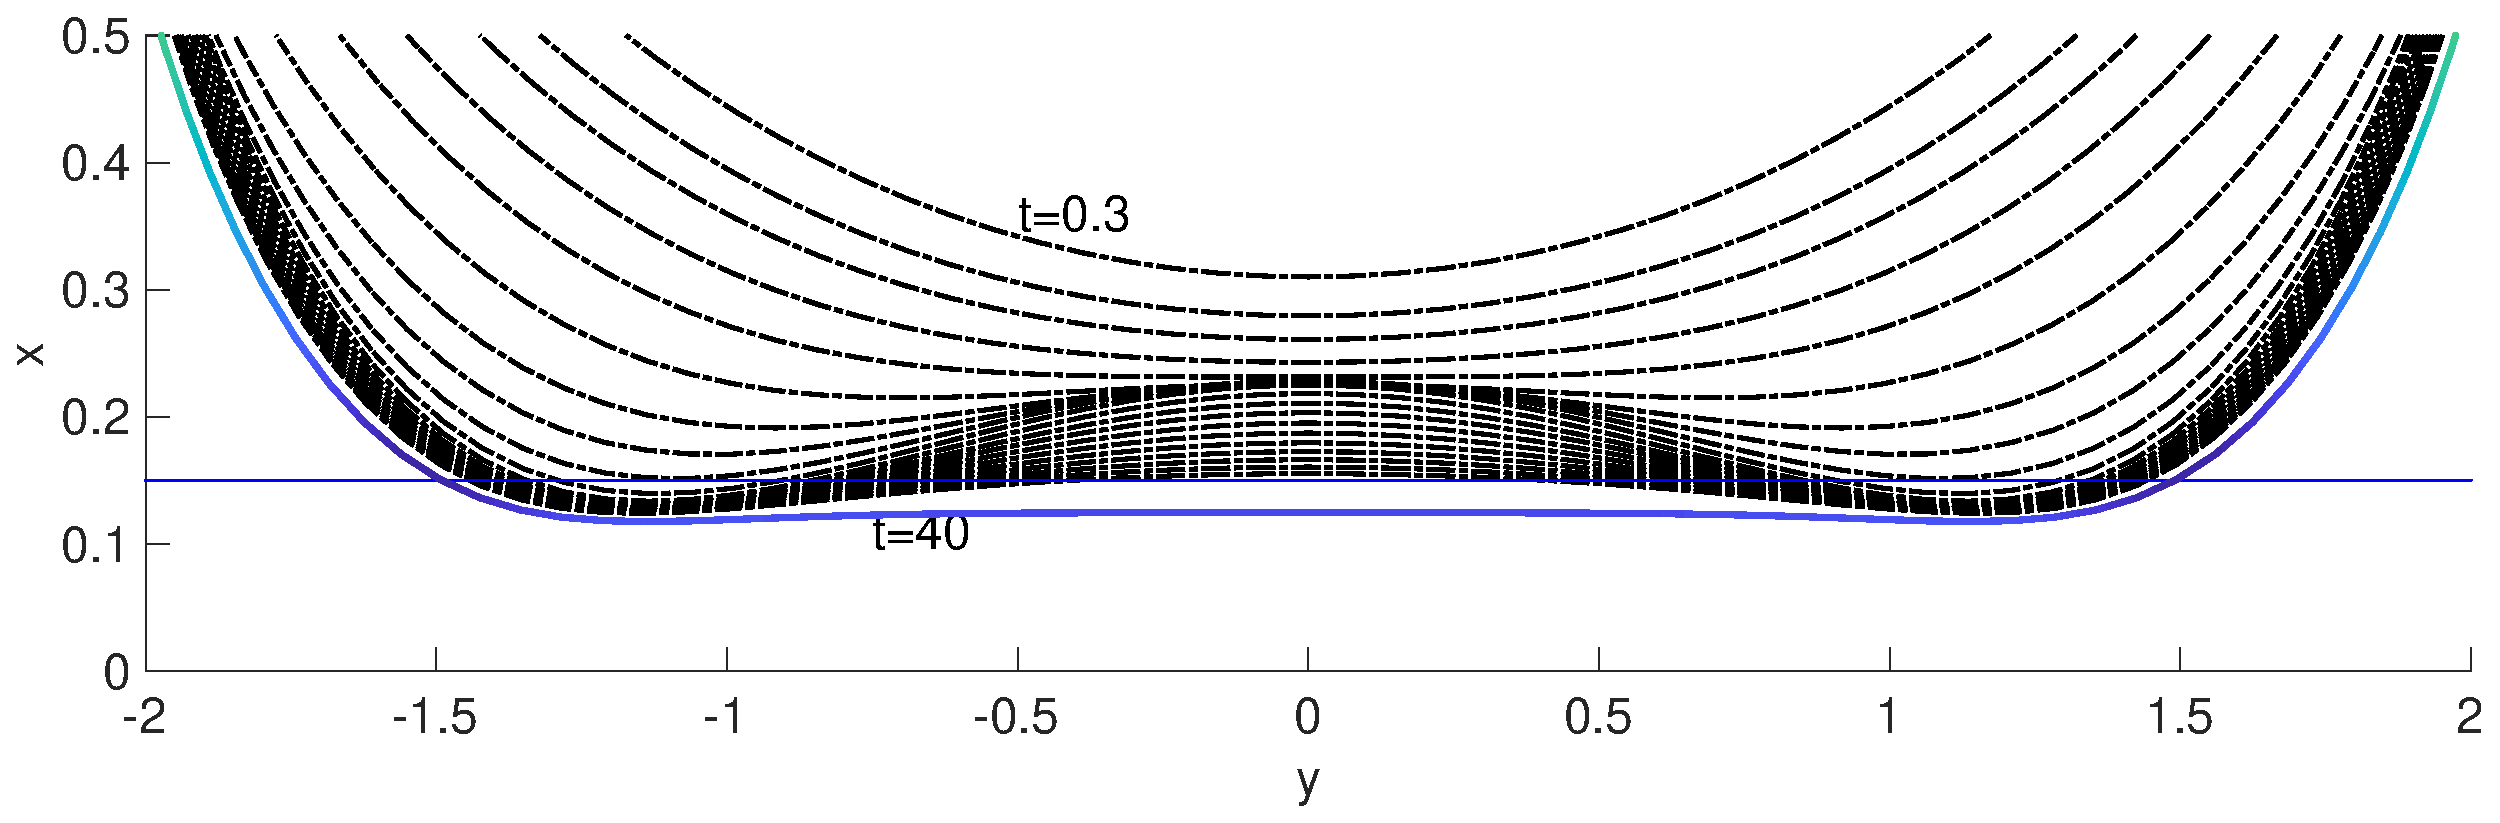
\includegraphics[keepaspectratio=true,scale=0.4]{figs/relax2Ves01g-draining01a.eps}
%% \caption{Adhesion dynamics of two vesicles with $\delta = 0.3$. From $t=0.3$ to $t=40$, the time interval $\delta t = 0.3$ between every two neighboring dash-dotted curves.}
%% \label{fig:qflow_g-draining01a}
%% \end{figure}
%
%% \begin{figure}
%% 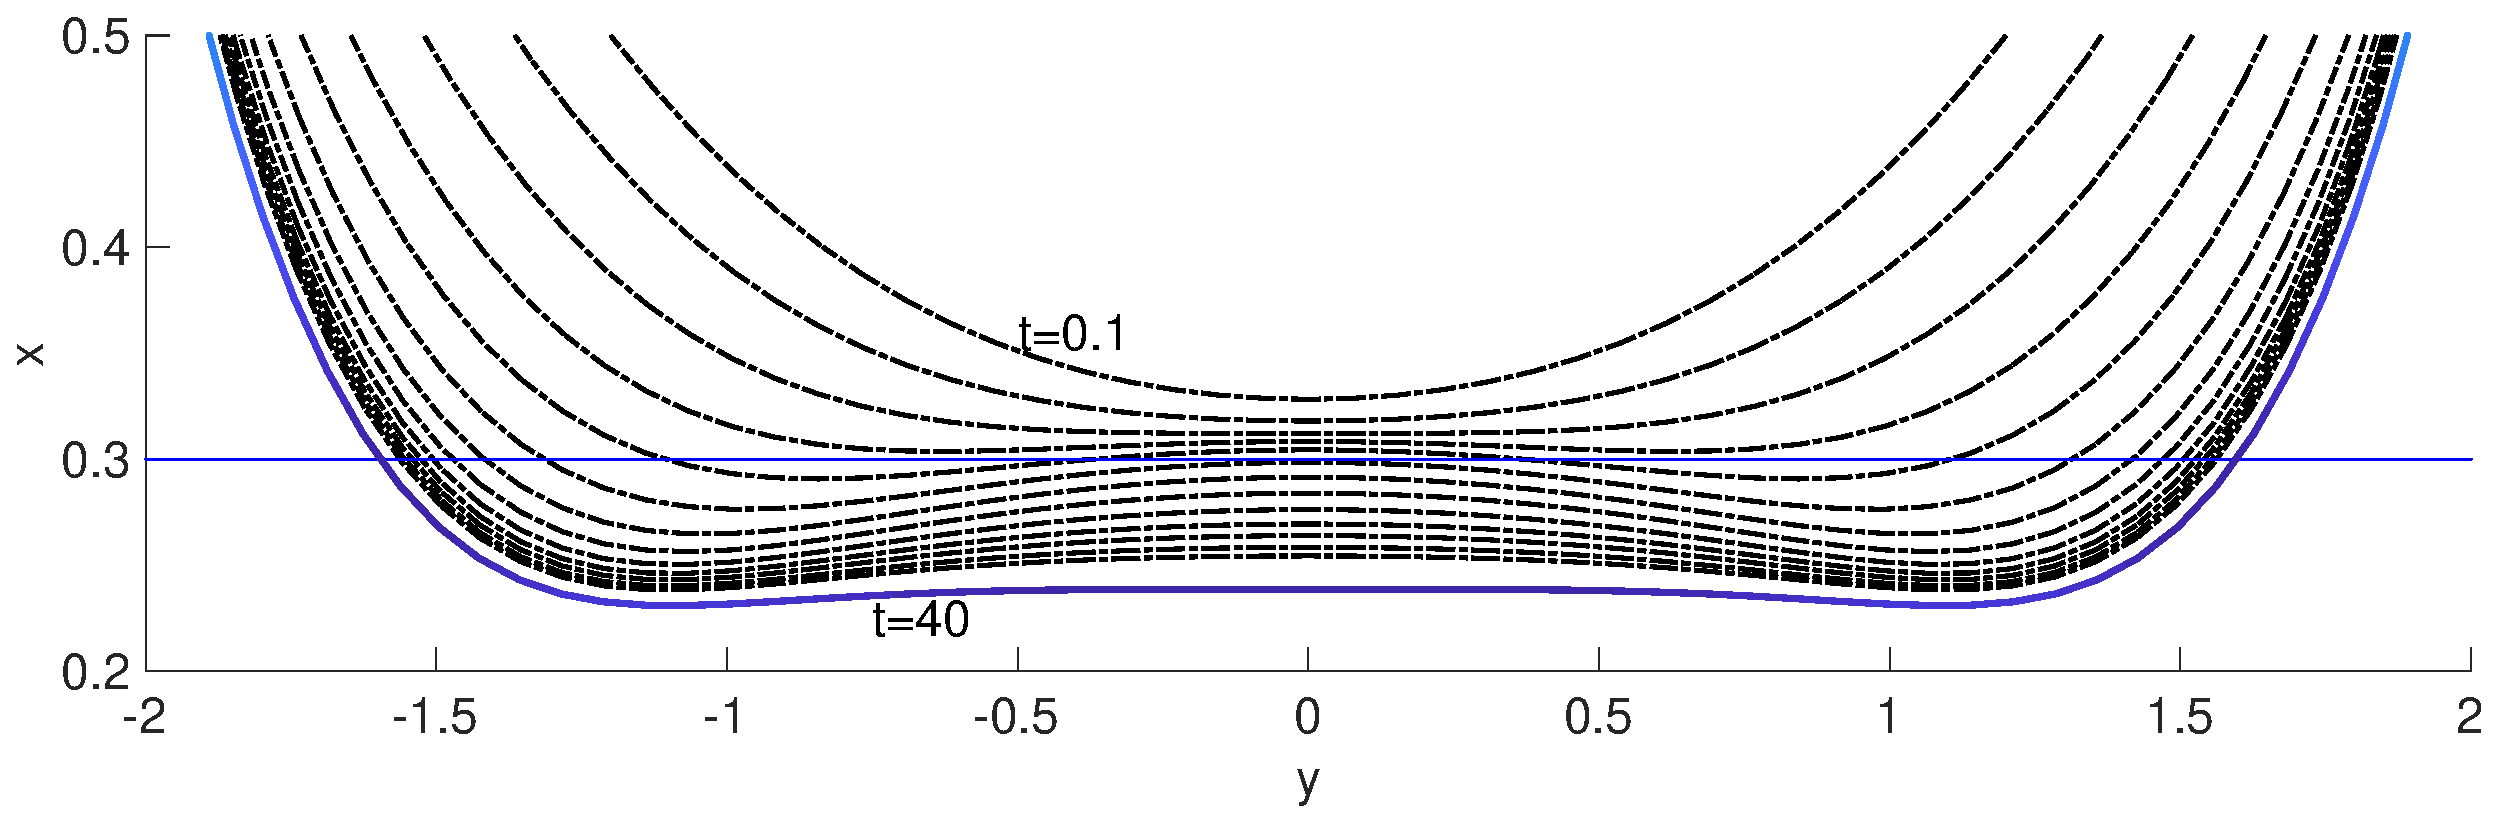
\includegraphics[keepaspectratio=true,scale=0.4]{figs/relax2Ves01j-draining01a.eps}
%% \caption{Adhesion dynamics of two vesicles with $\delta = 0.6$. From $t=0.1$ to $t=40$, the time interval $\delta t = 0.1$ between every two neighboring dash-dotted curves.}
%% \label{fig:qflow_g-draining01a}
%% \end{figure}
%
%%%%%%%%%%%%%%%%%%%%%%%%%%%%%%%%%%%%%%%%%%%%%%%%%%%%%%%%%%%%%%%%%%%%%%%%%
%\subsection{Effects of reduced area}
%\label{sec:qflow_reduced_area} 
%Figure~\ref{fig:qflow_reduced_area}
%
%\begin{figure}
%\includegraphics[keepaspectratio=true,scale=0.5]{figs/nrelax2Ves02o_rA.png}
%\caption{The effect of the reduced area on adhering vesicles in a
%quiescent flow.  The parameters of the vdW potential are $\delta = 0.2$
%and $\sigma = 0.5$.}
%\label{fig:qflow_reduced_area}
%\end{figure}
%
%% \begin{figure}
%% 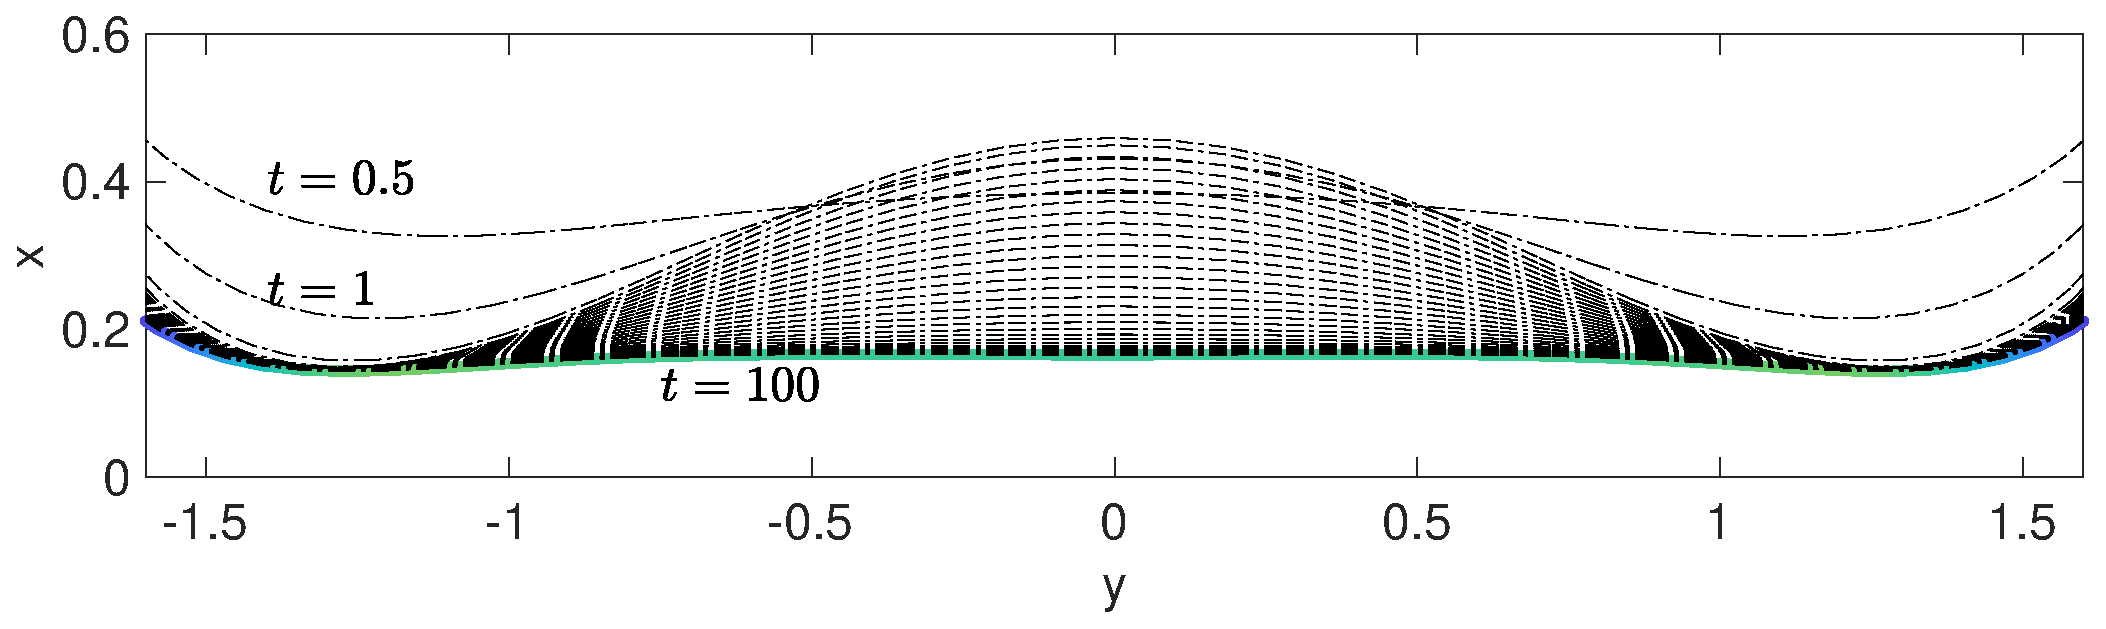
\includegraphics[keepaspectratio=true,scale=0.4]{figs/relax2Ves01usa.eps}
%% \caption{Adhesion dynamics of two vesicles with $\delta = 0.4$ and $\sigma=0.2$. From $t=0.06$ to $t=100$, the time interval $\delta t = 0.06$ between every two neighboring dash-dotted curves.}
%% \label{fig:qflow_u-draining}
%% \end{figure}
%
%% \begin{figure}
%% 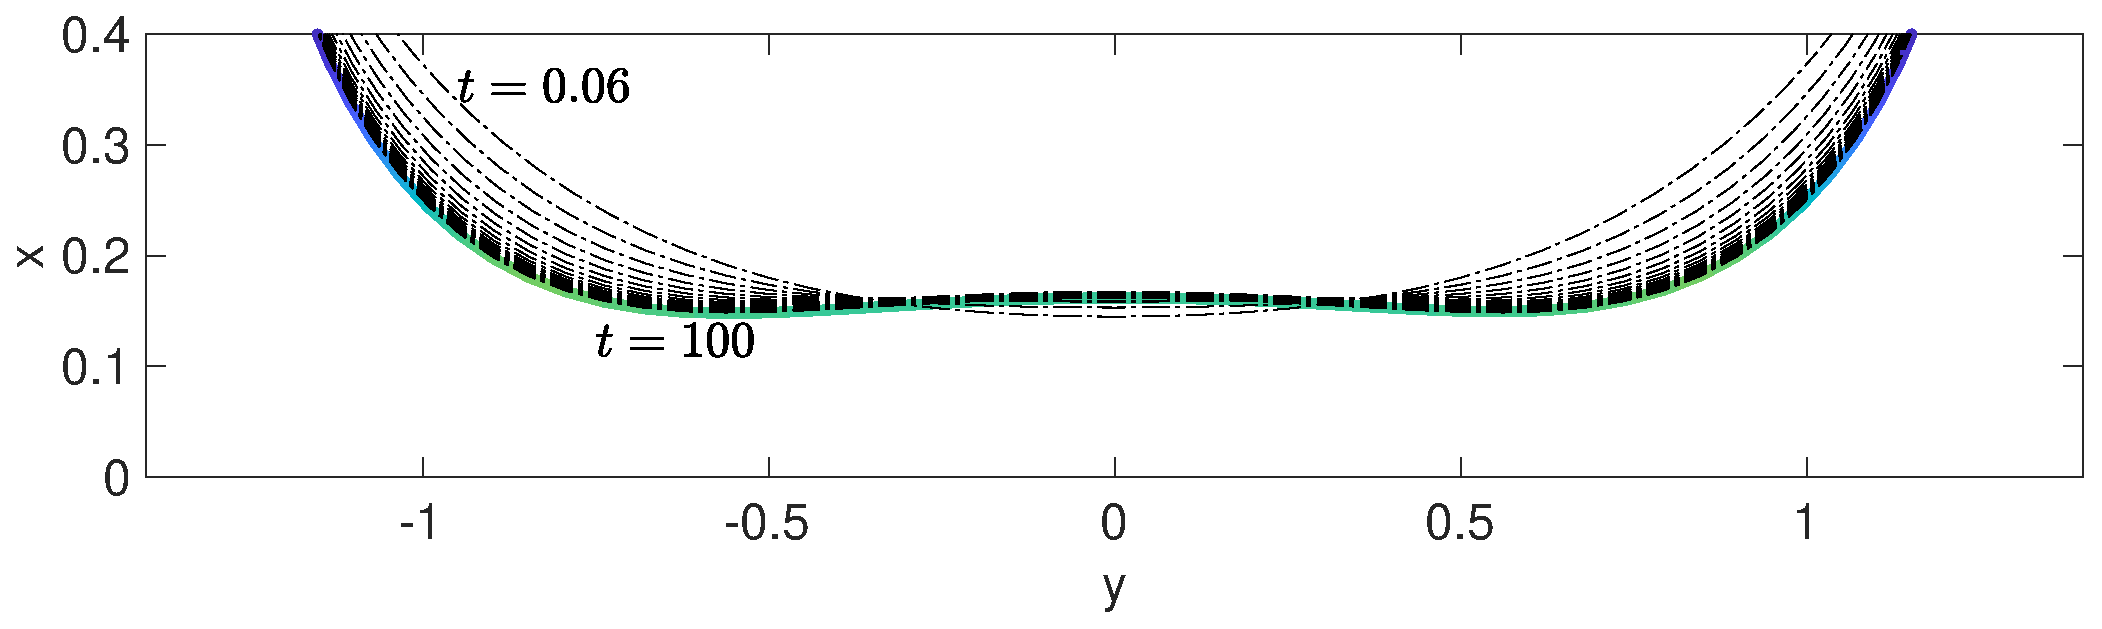
\includegraphics[keepaspectratio=true,scale=0.4]{figs/relax2Ves01zsa.eps}
%% \caption{Adhesion dynamics of two vesicles with $\delta = 0.4$ and $\sigma=0.2$. From $t=1$ to $t=100$, the time interval $\delta t = 1$ 
%% between every two neighboring dash-dotted curves.}
%% \label{fig:qflow_z-draining}
%% \end{figure}

%%%%%%%%%%%%%%%%%%%%%%%%%%%%%%%%%%%%%%%%%%%%%%%%%%%%%%%%%%%%%%%%%%%%%%%%
\section{Adhesion of two vesicles in an extensional flow} 
\label{sec:eflow} 
The hydrodynamics of a single vesicle in an 
extensional flow has revealed novel nonlinear vesicle dynamics not found for a viscous drop \cite{KantslerSegreSteinberg2008_PRL,ZhaoShaqfeh2013_JFM,Narsimhan2014_JFM,DahlNarsimhanGouveia2016_SoftMatt}.
The stagnation point (zero-velocity point) in an extensional flow is a saddle point where two laminar streams converge along an axis and then diverge in a
different direction. 
With an active control algorithm to fix the position of the stagnation point by adjusting the streaming flow strength with a feedback loop \cite{Johnson-Chavarria2011_EMJ},
a particle can be trapped at the stagnation point for long time scales to facilitate
image acquisition or other detailed measures such as PIV of flow inside/around the particle.
To explore the application of such fluid trap to measure the adhesion strength between two bound vesicle membranes, we propose the following thought experiment.


We begin from two vesicles forming a doublet under an adhesion potential in a quiescent flow as in \S~\ref{sec:qflow}. 
Once a doublet forms and reaches an equilibrium configuration, we turn on 
the fluid trap with the stagnation point placed at the center of the vesicle doublet.
For simplification we assume that each vesicle in the doublet has the same reduced area, membrane area, and bending stiffness.
At low extensional rate, we expect the vesicle doublet to stay bound at the fluid trap stagnation point.
On the other hand, the vesicle doublet may become unstable and eventually separate at a high extensional rate.
Thus we expect there to exist a critical extensional rate above which the vesicle doublet cannot stay bound under a given adhesion potential.
The dependence of the critical extensional rate on the adhesion potential and the mechanical vesicle properties thus provides a means to probe the physics of membrane adhesion.


We consider two vesicles suspended in the extensional flow $\uu =
\chi(-x,y)$, where $\chi$ is the extensional rate.  The vesicles are
initially placed symmetrically on the $x$ axis in a quiescent flow
($\chi = 0$).  Once they reach steady-state doublet, the extensional
background flow is started.  We use this example to characterize the
required extensional rate to overcome the adhesive forces of the
doublet.  In particular, we investigate the effect of the reduced area.
For all the simulations, the length of the vesicles are fixed, while the
area is changed to achieve the desired reduced area.

We observe three different vesicle configurations that depend on the
reduced area and extensional rate.  First, the doublet is not broken and
the individual vesicles long axis is parallel to the contracting
direction (Figure~\ref{fig:extensional1}).  Second, the doublet is not
broken, but it tilts to some inclination angle that is not parallel to
either of the contracting or separation directions
(Figure~\ref{fig:extensional3}).  Finally, if the extensional rate is
sufficiently large, the doublet is broken and the vesicles tend to
$(0,\pm \infty)$.


\begin{figure}[htp]
  \includegraphics[width = 0.19\textwidth]{figs/extensional_adR4em1adS7em1Chi2em2_ra070_image01.png}
  \includegraphics[width = 0.19\textwidth]{figs/extensional_adR4em1adS7em1Chi2em2_ra070_image02.png}
  \includegraphics[width = 0.19\textwidth]{figs/extensional_adR4em1adS7em1Chi2em2_ra070_image03.png}
  \includegraphics[width = 0.19\textwidth]{figs/extensional_adR4em1adS7em1Chi2em2_ra070_image04.png}
  \includegraphics[width = 0.19\textwidth]{figs/extensional_adR4em1adS7em1Chi2em2_ra070_image05.png}
  \caption{\label{fig:extensional1} Two vesicles in an extensional flow.
  The reduced area is $0.7$, the adhesion strength is $0.7$, and the
  adhesion length scale is $0.4$, extensional rate is $\chi = 0.02$.
  The doublet tilts to an inclination angle.
  }
\end{figure}


\begin{figure}[htp]
  \includegraphics[width = 0.19\textwidth]{figs/extensional_adR4em1adS7em1Chi7em2_ra070_image01.png}
  \includegraphics[width = 0.19\textwidth]{figs/extensional_adR4em1adS7em1Chi7em2_ra070_image02.png}
  \includegraphics[width = 0.19\textwidth]{figs/extensional_adR4em1adS7em1Chi7em2_ra070_image03.png}
  \includegraphics[width = 0.19\textwidth]{figs/extensional_adR4em1adS7em1Chi7em2_ra070_image04.png}
  \includegraphics[width = 0.19\textwidth]{figs/extensional_adR4em1adS7em1Chi7em2_ra070_image05.png}
  \caption{\label{fig:extensional2} Two vesicles in an extensional flow.
  The reduced area is $0.7$, the adhesion strength is $0.7$, and the
  adhesion length scale is $0.4$, extensional rate is $\chi = 0.07$.
  The doublet tilts to an inclination angle.}
\end{figure}


\begin{figure}[htp]
  \includegraphics[width = 0.19\textwidth]{figs/extensional_adR4em1adS7em1Chi1em1_ra070_image01.png}
  \includegraphics[width = 0.19\textwidth]{figs/extensional_adR4em1adS7em1Chi1em1_ra070_image02.png}
  \includegraphics[width = 0.19\textwidth]{figs/extensional_adR4em1adS7em1Chi1em1_ra070_image03.png}
  \includegraphics[width = 0.19\textwidth]{figs/extensional_adR4em1adS7em1Chi1em1_ra070_image04.png}
  \includegraphics[width = 0.19\textwidth]{figs/extensional_adR4em1adS7em1Chi1em1_ra070_image05.png}
  \caption{\label{fig:extensional3} Two vesicles in an extensional flow.
  The reduced area is $0.7$, the adhesion strength is $0.7$, and the
  adhesion length scale is $0.4$, extensional rate is $\chi = 0.1$.  The
  vesicles extensional rate has overcome the adhesive force, and the
  vesicles doublet is broken.}
\end{figure}

Whether the doublet is broken or not and the inclination angle of the
doublet depends on the extensional rate and the vesicles' reduced area.
A phase diagram of the steady-state configuration is in
Figure~\ref{fig:extensionalPhaseDiagram}.  Final configurations that
remain symmetric to the flow (Figure~\ref{fig:extensional1} are
indicated by red dots, tilt to some inclination angle
(Figure~\ref{fig:extensional2} are indicated by blue dots, and that
separate (Figure~\ref{fig:extensional3}) are indicated by green dots.


\begin{figure}[htp]
  \includegraphics[width=0.5\textwidth]{figs/extensional_adR4em1adS7em1_phaseDiagram.pdf}
  \caption{\label{fig:extensionalPhaseDiagram} Phase diagram of vesicle
  hydrodynamics in an extensional flow.  At a fixed Hamaker constant
  $\sigma=0.7$ and adhesion length scale $\delta=0.4$, doublets may
  either remain symmetric to the flow (red marks), or tilt to some
  inclination angle (blue dots), or the extensional rate, $\chi$, may
  overcome the adhesive force (green dots).}
\end{figure}

In Figure~\ref{fig:extensionalInclinationAngle}, we plot the inclination
angle of a doublet formed by two vesicles of reduced area $0.70$ at four
different extensional rates.  

\begin{figure}[htp]
  \centering
  \includegraphics[height=0.4\textwidth]{figs/adR4em1adS7em1_ra070_inclinationAngle.pdf}
  \hfill
  \includegraphics[height=0.4\textwidth]{figs/angleDefinition.pdf}
  \caption{\label{fig:extensionalInclinationAngle} {\em Left}: The
  inclination angle of a doublet formed by vesicles of reduced area
  $0.70$ submerged in an extensional flow with an extensional rate of
  $\chi$. {\em Right}: The definition of the inclination angle.  An
  inclination angle of $\pi$ indicates a doublet whose long axis is
  parallel to the converging direction, while an inclination angle of
  $\pi/2$ indicates a doublet whose short axis is parallel to the
  converging direction.}
\end{figure}


%%%%%%%%%%%%%%%%%%%%%%%%%%%%%%%%%%%%%%%%%%%%%%%%%%%%%%%%%%%%%%%%%%%%%%%%
\section{Adhesion of two vesicles in a shear flow}
\label{sec:sflow} 
We consider two vesicles suspended in the shear flow $\uu = \chi(y,0)$,
where $\chi$ is the shear rate.  The vesicles are placed on the $y$ axis
so that the background velocity drives the vesicles towards one another.
In the absence of adhesion, once the vesicles are sufficiently close,
they are deflected to opposite sides of the $y$ axis, and the result is
that the distance between the vesicles goes to infinity.  However, in
the presence of adhesion, is it possible that the adhesive force keeps
the vesicles from separating, resulting in the formation of a {\em
doublet}~\cite{}.

The formation of the doublet depends on four main parameters: the
vesicles' reduced area, the adhesion length scale $\delta$, the adhesion
strength $\sigma$, and the shear rate $\chi$.
Figure~\ref{fig:doublet090} shows the configuration of two vesicles that
have formed a doublet at several instances in time.  In
Figure~\ref{fig:sflow_phase_diagram} (left), we show the minimum
distance between the two vesicles as a function of time for various
adhesion strengths.  The adhesion strength corresponding to the red
curves is less than a critical strength $\sigma_c$ for a doublet to
form.  In contrast, for larger adhesive strengths, doublets are formed
(blue curves).

\begin{figure}[htp]
  \includegraphics[width=0.24\textwidth]{figs/adR4em1adS7em1Chi5em1_ra090_image01.png}
  \includegraphics[width=0.24\textwidth]{figs/adR4em1adS7em1Chi5em1_ra090_image02.png}
  \includegraphics[width=0.24\textwidth]{figs/adR4em1adS7em1Chi5em1_ra090_image03.png}
  \includegraphics[width=0.24\textwidth]{figs/adR4em1adS7em1Chi5em1_ra090_image04.png}
  \includegraphics[width=0.24\textwidth]{figs/adR4em1adS7em1Chi5em1_ra090_image05.png}
  \includegraphics[width=0.24\textwidth]{figs/adR4em1adS7em1Chi5em1_ra090_image06.png}
  \includegraphics[width=0.24\textwidth]{figs/adR4em1adS7em1Chi5em1_ra090_image07.png}
  \includegraphics[width=0.24\textwidth]{figs/adR4em1adS7em1Chi5em1_ra090_image08.png}
  \caption{\label{fig:doublet090} The formation of a doublet in a shear
  flow.  The reduced area is $0.90$, the Hamaker contsant is $\sigma=0.7$, the
adhesion length scale is $\delta = 0.4$, and the shear rate is $\chi=0.5$.}
\end{figure}

\begin{figure}
  \includegraphics[height=0.4\textwidth]{figs/shear_adR4em1Chi1e0_ra-090.pdf}
  \includegraphics[height=0.4\textwidth]{figs/shear_adR4em1_ra090_phaseDiagram.pdf}
  \caption{{\em Left}: Distance between a pair of vesicles in a planar
    shear flow with shear rate $\chi=0.5$ and adhesion length scale
    $\delta = 0.4$.   The different lines correspond to a linear spacing
    of adhesion strengths ranging from $\sigma=0.1$ and $\sigma=1.0$.
    {\em Right}: Phase diagram of vesicle hydrodynamics in a shear flow.
    At a fixed reduced area $\triangle A=0.90$ and $\delta =0.4$,  the
    critical vdW potential strength $\sigma$ for binding of two vesicles
  in a shear flow depends on the shear rate $\chi$.
\label{fig:sflow_phase_diagram}}
\end{figure}

%Figures~\ref{fig:sflow_phase_diagram},
%~\ref{fig:sflow_1frames}, and~\ref{fig:sflow_2frames}
%\begin{figure}
%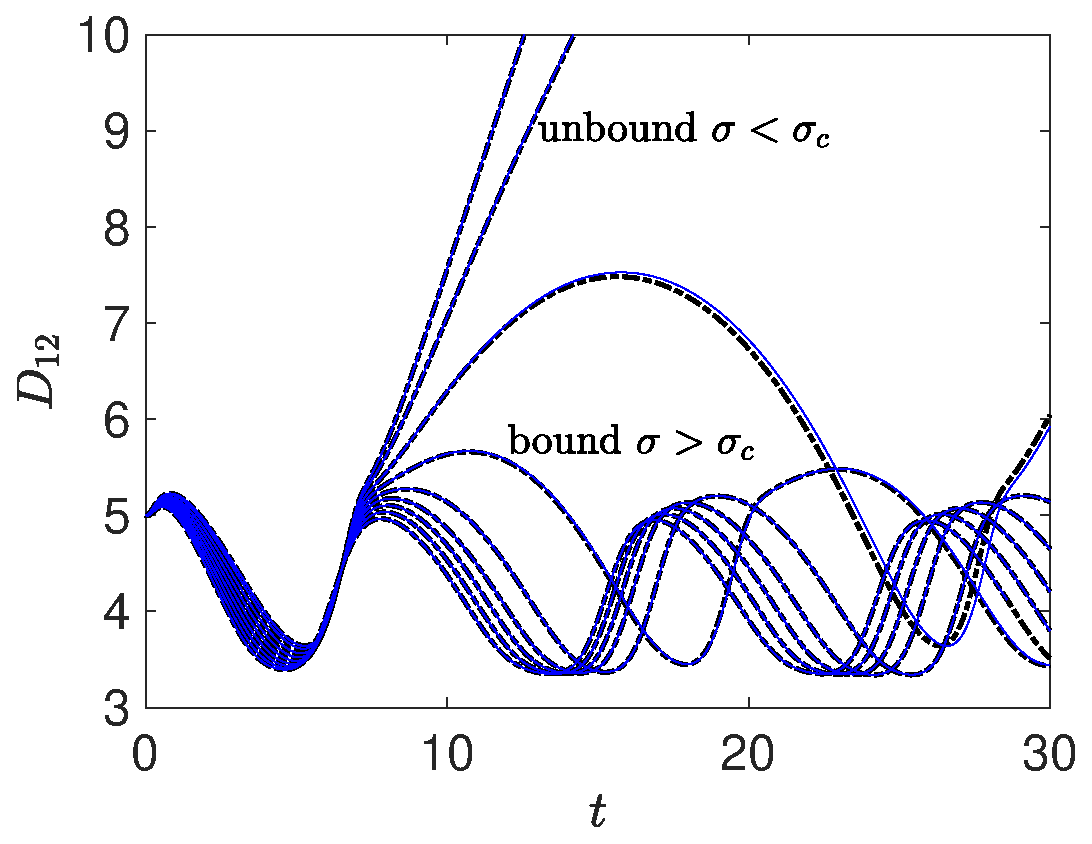
\includegraphics[keepaspectratio=true,scale=0.41]{figs/shear2Ves01a-iD12a.eps}
%\includegraphics[keepaspectratio=true,scale=0.415]{Nshear02_adS_ShearRate01.png}
%% \includegraphics[keepaspectratio=true,scale=0.40]{figs/Nshear02_adS_rA01.png}
%\caption{(a) Dynamics of a pair of vesicles in a planar shear flow with shear rate $\dot\gamma=1$ and vdW length $\delta = 0.4$. (b) Phase diagram of vesicle hydrodynamics in a shear flow. At a fixed reduced area $\triangle A=0.95$ and $\delta =0.4$,  the critical vdW potential strength $\sigma$ for binding of two vesicles in a shear flow depends on the shear rate $\dot\gamma$.}
%\label{fig:sflow_phase_diagram}
%\end{figure}

We investigate rheology of suspensions by computing the effective
viscosity of a doublet and compare it to the effective viscosity of a
single tank-treading vesicle. The effective viscosity is defined as the
viscosity of a homogeneous Newtonian fluid with the same energy
dissipation per macroscopic element of fluid.  In a simple shear flow,
the ambient velocity field is given by $\uu(\xx) = \chi(y,0)$, where
$\chi$ is the shear rate, and the intrinsic viscosity is
\begin{align*}
  [\mu]:= \frac{\mu_{\mathrm{eff}} - \mu_0}{\phi \mu_0} = 
  \frac{1}{\chi \mu_0 T} \int_{T_i}^{T_e} 
  \langle \sigma_{12} \rangle dt,
\end{align*}
where
\begin{align*}
  \langle \sigma \rangle = \frac{1}{|\omega|} \int_{\gamma}
    \xxi \otimes \xx ds.
\end{align*}
Here, $[\mu]$ is the intrinsic viscosity, $\phi$ is the area fraction of
vesicles, $\sigma$ is the stress due to the vesicles, and $\langle \cdot
\rangle$ is the spatial average.

In the left plot of Figure~\ref{fig:shearIntrinsicViscosity}, we compare
the intrinsic viscosity of a single tank treading vesicle to a doublet.
To validate our simulations, we superimpose (black marks) the intrinsic
viscosity calculated by Ghigliotti et
al.~\cite{GhigliottiBibenMisbah2010_JFM}.  The presence of the doublet
significantly increases the intrinsic viscosity at all the reduced
areas.  To further characterize the effect of adhesion, in the right
plot of Figure~\ref{fig:shearIntrinsicViscosity} we decompose the
intrinsic viscosity into the contributions from the bending and tension
(blue), and the contribution from the adhesion (red).  We also
superimpose twice the intrinsic viscosity of a single tank treading
vesicle (dashed curve) to demonstrate that the bending and tension of
the doublet behaves similarly, but not identically, to a dilute
suspensions of non-adhering tank-treading vesicles.  We see that the
effect of the adhesion on the intrinsic viscosity is largest for
vesicles with small reduced areas.

\begin{figure}[htp]
  \centering
  \includegraphics[width=0.45\textwidth]{figs/shear2Ves_adR4em1adS7em1Chi5em1.pdf}
  \includegraphics[width=0.45\textwidth]{figs/doublet_decomp.pdf}
  \caption{\label{fig:shearIntrinsicViscosity} {\em Left}: The intrinsic
  viscosity of a tank treading vesicle (blue) and a doublet (red).  The
  shear rate is $\chi = 0.5$, the Hamaker constant is $\sigma = 0.7$,
  and the adhesion length scale is $\delta = 0.4$.  The length of the
  vesicles at each of the reduced areas is fixed, while the area changes
  with differing reduced areas.  The black marks denote intrinsic
  viscosity values computed by Ghigliotti et
  al.~\cite{GhigliottiBibenMisbah2010_JFM} (cf.~Figure 5).  {\em Right}:
  The decomposition of the intrinsic viscosity into the contributions
  for the bending and tension (blue) of the vesicles, and the
  contribution from the vesicle adhesion (red).  Also included is twice
  the intrinsic viscosity of a single tank-treading vesicle.}
\end{figure}



%%%%%%%%%%%%%%%%%%%%%%%%%%%%%%%%%%%%%%%%%%%%%%%%%%%%%%%%%%%%%%%%%%%%%%%%
\section{Conclusions}
\todo[inline]{Concluding remarks}

Future work includes three dimensional simulations, viscosity contrast,
confined suspensions, and dense suspensions.

Recently Liu {\it et al.} \cite{LiuChuNewbyRead2018_bioRxiv} used
immersed boundary simulations to show that, at a separation distance of
tens of nanometers, the thin film between the two membranes facilitate
the coupling between membranes via strong hydrodynamic interactions. In
particular they demonstrate numerically that the fluctuation in one
membrane is highly correlated to the other membrane without any physical
contact. It is not clear how thermal fluctuations may affect the
hydrodynamics of vesicles under adhesion. For example, does the
fluctuating hydrodynamics in the thin film between two vesicles enhance
adhesion to keep vesicles bound under linear flows?

\begin{appendices}
\section{Adhesion Force}
\label{sec:appendixA}
Consider a suspension of two vesicles $\gamma_1$ and $\gamma_2$
parameterized as $\xx_1(s)$ and $\xx_2(s)$, respectively, with $s \in
[0,1]$.  Here $s$ is the arclength, and we have assumed, without loss of
generality, that both vesicles have length one.  We use the van der
Waals potential
\begin{align*}
  \phi(z) = \sigma \left[ 
    \left(\frac{\delta}{z}\right)^m - \frac{m}{n}\left(\frac{\delta}{z}\right)^n \right],
\end{align*}
where $z$ is the distance between two points.  Then, we define the total
adhesive energy on $\gamma_1$ to be
\begin{align*}
  U_1 = \int_{\gamma_1} \int_{\gamma_2} \phi(\|\xx_1 - \xx_2\|) 
    ds_{\xx_2} ds_{\xx_1}
\end{align*}
Perturbing $\xx_1$ to $\tilde{\xx}_1 = \xx_1 +  \delta \xx_1$, results
in a new vesicle $\tilde{\gamma}_1$, and the perturbed adhesive energy is
\begin{align*}
  \widetilde{U}_1 = \int_{\tilde{\gamma}_1} \int_{\gamma_2}
  \phi(\|\tilde{\xx}_1 - \xx_2\|) ds_{\xx_2} ds_{\tilde{\xx}_1},
\end{align*}
and the change in the energy is
\begin{align*}
  \delta U_1 = \int_{\tilde{\gamma}_1} \int_{\gamma_2}
  \phi(\|\tilde{\xx}_1 - \xx_2\|) ds_{\xx_2} ds_{\tilde{\xx}_1} - 
  \int_{\gamma_1} \int_{\gamma_2} \phi(\|\xx_1 - \xx_2\|) 
  ds_{\xx_2} ds_{\xx_1}.
\end{align*}

We now decompose the perturbation into normal and tangential components
as $\delta \xx_1 = \epsilon \yy(s) = \epsilon(u\tt + v\nn)$. The
perturbed arclength term, to leading order, is
\begin{align*}
  \|\tilde{\xx}'_1\| \approx 1 + \epsilon(u_s + \nu\kappa),
\end{align*}
where $\kappa$ is the curvature.  To leading order, inextensible
perturbations satisfy $u_s + \kappa v = 0$, so the arclength term of
$\gamma_1$ and $\tilde{\gamma}_1$ are identical to leading order.
Therefore,
\begin{align*}
  \delta U_1 &= \int_{\gamma_1} \int_{\gamma_2} \left(
  \phi(\|\xx_1 + \epsilon \yy  - \xx_2\|) - \phi(\|\xx_1 - \xx_2\|)
  \right) ds_{\xx_2} ds_{\xx_1} \\
  &\approx \epsilon \int_{\gamma_1} \int_{\gamma_2}
  \nabla \phi (\|\xx_1 - \xx_2\|) \cdot \yy ds_{\xx_2} ds_{\xx_1}
\end{align*}
and the adhesive force applied by vesicle 2 on vesicle 1 is
\begin{align}
 \int_{\gamma_2}\nabla \phi(\|\xx_1 - \xx_2\|)ds_{\xx_2} = -m \sigma\delta^{n}
   \int_{\gamma_k} \frac{\xx - \yy}{\|\xx - \yy\|^{m+2}} 
  \left(\delta^{m-n} - \|\xx - \yy\|^{m-n} \right) ds_\yy.
  \end{align}
When $(m,n) = (4,2)$, the above express becomes
\begin{align*}
  \int_{\gamma_2}\nabla \phi(\|\xx_1 - \xx_2\|)ds_{\xx_2} = 
  -4 \sigma \delta^2 \int_{\gamma_2}
  \frac{\xx_1 - \xx_2}{\|\xx_1 - \xx_2\|^6} 
  \left(\delta^2 - \|\xx_1 - \xx_2\|^2 \right) ds_{\xx_2}.
\end{align*}
A similar expression holds for the adhesive force applied by vesicle 1
on vesicle 2, and equation~\eqref{eqn:adhesionForce} gives the adhesive
force for a suspension of $M$ vesicles.

%\section{Small Deformation Analysis on a Single Vesicle in Linear Shear Flow}
%\label{sec:appendixB}
%\todo[inline]{Used to validate the code/results}
%Hydrodynamics of a single vesicle in Stokes flow has been extensively investigated. 
%In a planar shear flow, the vesicle hydrodynamics is characterized by
%excess area (reduced volume), viscosity contrast between interior and exterior fluids, and shear rate of the imposed far-field fluid flow. 
%%In addition a vesicle with a rigid particle inside is also investigated as a biological mimic of a 
%%eukaryotic cell with a nucleus that occupies nearly half of the intracellular volume \cite{Veerapaneni2011_PRL}. 
%Small-deformation analysis shows that
%a vesicle tank-treads in a planar shear flow for low viscosity contrast and shear rate. At high viscosity contrast the tank-tread (TT) dynamics transitions to tumbling (TB) \cite{Misbah2006_PRL,Vlahovska2007_PRE} ,
%and this leads to a transition in effective shear viscosity in the vesicle suspension \cite{Misbah2006_PRL,Vitkova2008_BJ} that is also validated
%by direct numerical simulations \cite{GhigliottiBibenMisbah2010_JFM} and experiments \cite{KantslerSegreSteinberg2008_EPL,ZabuskySegreDeschamps2011_PoF}.
%Between TT and TB vesicle hydrodynamics, a breathing (tremble) is also observed \cite{Misbah2006_PRL,KantslerSegreSteinberg2008_PRL,ZhaoShaqfeh2011_JFM,SpannZhaoShaqfeh2014_PoF} to affect the effective shear viscosity in a 
%different way.
%Some of these theoretical results have inspired detailed comparison of rheology of a dilute vesicle suspension between direct numerical simulations and experiments.
%Here we follow the small-deformation analysis by Finken {\it et al.} to derive the effective shear viscosity of a dilute suspension of TT vesicle in a planar shear flow.
%The main results in the derivation carried out in the Mathematica run script (supplementary material) are summarized here.
%For the homogeneous membrane tension of an inextensible two-dimensional vesicle (with an excess length $\triangle$) under a planar shear flow we found
%\begin{equation}
%\sigma_0 = -\frac{5}{2} + 
%\end{equation}
%
%The effective shear viscosity of a single TT vesicle in a planar shear flow has been 
%
% studied and comparison between numerical simulations, small-deformation theory and experiments has been made.
%Following the asymptotic analysis by Finken {\it et al.} \cite{Finken2008_EPL} we 
%In an extensional flow (planar or uniaxial), vesicle shape dynamics
%depends sensitively on the vesicle reduced volume  and the elastic capillary number \cite{KantslerSegreSteinberg2008_PRL,ZhaoShaqfeh2013_JFM,Narsimhan2014_JFM,DahlNarsimhanGouveia2016_SoftMatt}: Asymmetric shape and oscillatory undulation of the vesicle membrane are two examples of the complex vesicle hydrodynamics in an extensional flow.




\end{appendices}


\bibliography{refs}
%%%%%%%%%%%%%%%%%%%%%%%%%%%%%%%%%%%%%%%%%%%%%%%%%%%%%%%%%%%%%%%%%%%%%%%%%%%%%%%
%\subsection{\label{sec:level2}Second-level heading: Formatting}
%
%This file may be formatted in either the \texttt{preprint} or
%\texttt{reprint} style. \texttt{reprint} format mimics final journal output. 
%Either format may be used for submission purposes. \texttt{letter} sized paper should
%be used when submitting to APS journals.
%
%%%%%%%%%%%%%%%%%%%%%%%%%%%%%%%%%%%%%%%%%%%%%%%%%%%%%%%%%%%%%%%%%%%%%%%%%%%%%%%
%\subsubsection{Wide text (A level-3 head)}
%The \texttt{widetext} environment will make the text the width of the
%full page, as on page~\pageref{eq:wideeq}. (Note the use the
%\verb+\pageref{#1}+ command to refer to the page number.) 
%\paragraph{Note (Fourth-level head is run in)}
%The width-changing commands only take effect in two-column formatting. 
%There is no effect if text is in a single column.

%%%%%%%%%%%%%%%%%%%%%%%%%%%%%%%%%%%%%%%%%%%%%%%%%%%%%%%%%%%%%%%%%%%%%%%%%%%%%%
%\subsection{\label{sec:citeref}Citations and References}
%
%
%
%A citation in text uses the command \verb+\cite{#1}+ or
%\verb+\onlinecite{#1}+ and refers to an entry in the bibliography. 
%An entry in the bibliography is a reference to another document.

%%%%%%%%%%%%%%%%%%%%%%%%%%%%%%%%%%%%%%%%%%%%%%%%%%%%%%%%%%%%%%%%%%%%%%%%%%%%%%
%\subsubsection{Citations}


%Because REV\TeX\ uses the \verb+natbib+ package of Patrick Daly, 
%the entire repertoire of commands in that package are available for your document;
%see the \verb+natbib+ documentation for further details. Please note that
%REV\TeX\ requires version 8.31a or later of \verb+natbib+.
%
%\paragraph{Syntax}
%The argument of \verb+\cite+ may be a single \emph{key}, 
%or may consist of a comma-separated list of keys.
%The citation \emph{key} may contain 
%letters, numbers, the dash (-) character, or the period (.) character. 
%New with natbib 8.3 is an extension to the syntax that allows for 
%a star (*) form and two optional arguments on the citation key itself.
%The syntax of the \verb+\cite+ command is thus (informally stated)
%\begin{quotation}\flushleft\leftskip1em
%\verb+\cite+ \verb+{+ \emph{key} \verb+}+, or\\
%\verb+\cite+ \verb+{+ \emph{optarg+key} \verb+}+, or\\
%\verb+\cite+ \verb+{+ \emph{optarg+key} \verb+,+ \emph{optarg+key}\ldots \verb+}+,
%\end{quotation}\noindent
%where \emph{optarg+key} signifies 
%\begin{quotation}\flushleft\leftskip1em
%\emph{key}, or\\
%\texttt{*}\emph{key}, or\\
%\texttt{[}\emph{pre}\texttt{]}\emph{key}, or\\
%\texttt{[}\emph{pre}\texttt{]}\texttt{[}\emph{post}\texttt{]}\emph{key}, or even\\
%\texttt{*}\texttt{[}\emph{pre}\texttt{]}\texttt{[}\emph{post}\texttt{]}\emph{key}.
%\end{quotation}\noindent
%where \emph{pre} and \emph{post} is whatever text you wish to place 
%at the beginning and end, respectively, of the bibliographic reference
%(see Ref.~[\onlinecite{witten2001}] and the two under Ref.~[\onlinecite{feyn54}]).
%(Keep in mind that no automatic space or punctuation is applied.)
%It is highly recommended that you put the entire \emph{pre} or \emph{post} portion 
%within its own set of braces, for example: 
%\verb+\cite+ \verb+{+ \texttt{[} \verb+{+\emph{text}\verb+}+\texttt{]}\emph{key}\verb+}+.
%The extra set of braces will keep \LaTeX\ out of trouble if your \emph{text} contains the comma (,) character.
%
%The star (*) modifier to the \emph{key} signifies that the reference is to be 
%merged with the previous reference into a single bibliographic entry, 
%a common idiom in APS and AIP articles (see below, Ref.~[\onlinecite{epr}]). 
%When references are merged in this way, they are separated by a semicolon instead of 
%the period (full stop) that would otherwise appear.
%
%\paragraph{Eliding repeated information}
%When a reference is merged, some of its fields may be elided: for example, 
%when the author matches that of the previous reference, it is omitted. 
%If both author and journal match, both are omitted.
%If the journal matches, but the author does not, the journal is replaced by \emph{ibid.},
%as exemplified by Ref.~[\onlinecite{epr}]. 
%These rules embody common editorial practice in APS and AIP journals and will only
%be in effect if the markup features of the APS and AIP Bib\TeX\ styles is employed.
%
%\paragraph{The options of the cite command itself}
%Please note that optional arguments to the \emph{key} change the reference in the bibliography, 
%not the citation in the body of the document. 
%For the latter, use the optional arguments of the \verb+\cite+ command itself:
%\verb+\cite+ \texttt{*}\allowbreak
%\texttt{[}\emph{pre-cite}\texttt{]}\allowbreak
%\texttt{[}\emph{post-cite}\texttt{]}\allowbreak
%\verb+{+\emph{key-list}\verb+}+.

\end{document}
%
% ****** End of file apssamp.tex ******
